\label{sec:A}

\begin{figure}[h]
    \centering
    \begin{subfigure}[b]{0.55\linewidth}
        \centering
        \marginbox{0 0 0 0} {
            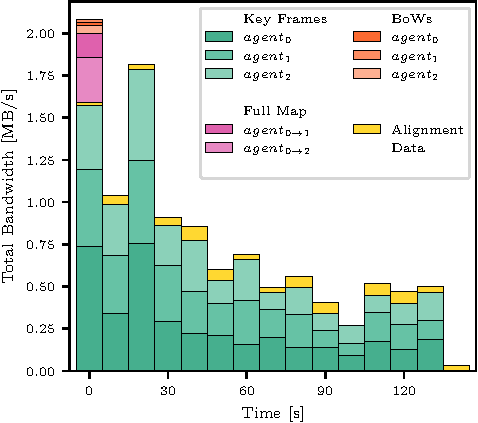
\includegraphics[width=\linewidth, valign=t]{figures/apr11_tum_room_trajectory_a_bandwith.pdf}
        }
        \caption{Total system data over time, segregated by message type}
    \end{subfigure}%
    ~
    \begin{subfigure}[b]{0.45\linewidth}
        \flushright
        \adjustbox{valign=t, width=\linewidth}{
            \marginbox{0.2in 0 0 0} {

                \def\arraystretch{1.2}
                \begin{tabular}{ |c|l|r|r| }
                    \cline{3-4}
                    \multicolumn{2}{}{}                       & \multicolumn{1}{|c|}{KB} & \multicolumn{1}{|c|}{Avg. KB/s}         \\
                    \hline
                    \multirow{3}{*}{Key Frames}               & $agent_0$                & 37,599                          & 264.9 \\
                                                              & $agent_1$                & 33,066                          & 233.0 \\
                                                              & $agent_2$                & 29,963                          & 211.1 \\
                    \hline
                    \multirow{3}{*}{BoWs}                     & $agent_0$                & 217                             & 1.5   \\
                                                              & $agent_1$                & 188                             & 1.3   \\
                                                              & $agent_2$                & 426                             & 3.0   \\
                    \hline
                    \multirow{2}{*}{Full Map}
                                                              & $agent_{0\to1}$          & 1,472                           & 10.4  \\
                                                              & $agent_{0\to2}$          & 2,631                           & 18.5  \\
                    \hline
                    \multicolumn{2}{|c|}{Alignment Data}      & 6,947                    & 49.0                                    \\
                    \hline
                    \multicolumn{2}{|c|}{\textbf{Total Data}} & \textbf{112,511}         & \textbf{792.8}                          \\
                    \hline
                \end{tabular}
            }
        }
        \caption{Total system data by message type}
        \vfill

        \adjustbox{valign=b, width=\linewidth}{
            \marginbox{0.2in 0 0 0.3in} {
                \def\arraystretch{1.2}
                \begin{tabular}{ |l|r|r|r|r| }
                    \cline{2-5}
                    \multicolumn{1}{}{} & \multicolumn{2}{|c|}{Sent} & \multicolumn{2}{|c|}{Received}                                                               \\
                    \cline{2-5}
                    \multicolumn{1}{}{} & \multicolumn{1}{|c|}{KB}   & \multicolumn{1}{|c|}{Avg. KB/s} & \multicolumn{1}{|c|}{KB} & \multicolumn{1}{|c|}{Avg. KB/s} \\
                    \hline
                    $agent_0$           & \textbf{49,083}            & \textbf{345.9}                  & \textbf{63,644}          & \textbf{448.5}                  \\
                    \hline
                    $agent_1$           & \textbf{33,254}            & \textbf{234.3}                  & \textbf{76,624}          & \textbf{539.9}                  \\
                    \hline
                    $agent_2$           & \textbf{30,389}            & \textbf{214.1}                  & \textbf{80,649}          & \textbf{568.3}                  \\
                    \hline
                \end{tabular}
            }
        }
        \caption{Data by agent}
    \end{subfigure}%

    \caption{Bandwidth used by the TUM-VI Rooms 01-03 scenarios running on my SLAM system.}
    \label{fig:tum-rooms-01-03-bandwith}
\end{figure}